\documentclass{article}\usepackage[]{graphicx}\usepackage[]{color}
%% maxwidth is the original width if it is less than linewidth
%% otherwise use linewidth (to make sure the graphics do not exceed the margin)
\makeatletter
\def\maxwidth{ %
  \ifdim\Gin@nat@width>\linewidth
    \linewidth
  \else
    \Gin@nat@width
  \fi
}
\makeatother

\definecolor{fgcolor}{rgb}{0.345, 0.345, 0.345}
\newcommand{\hlnum}[1]{\textcolor[rgb]{0.686,0.059,0.569}{#1}}%
\newcommand{\hlstr}[1]{\textcolor[rgb]{0.192,0.494,0.8}{#1}}%
\newcommand{\hlcom}[1]{\textcolor[rgb]{0.678,0.584,0.686}{\textit{#1}}}%
\newcommand{\hlopt}[1]{\textcolor[rgb]{0,0,0}{#1}}%
\newcommand{\hlstd}[1]{\textcolor[rgb]{0.345,0.345,0.345}{#1}}%
\newcommand{\hlkwa}[1]{\textcolor[rgb]{0.161,0.373,0.58}{\textbf{#1}}}%
\newcommand{\hlkwb}[1]{\textcolor[rgb]{0.69,0.353,0.396}{#1}}%
\newcommand{\hlkwc}[1]{\textcolor[rgb]{0.333,0.667,0.333}{#1}}%
\newcommand{\hlkwd}[1]{\textcolor[rgb]{0.737,0.353,0.396}{\textbf{#1}}}%
\let\hlipl\hlkwb

\usepackage{framed}
\makeatletter
\newenvironment{kframe}{%
 \def\at@end@of@kframe{}%
 \ifinner\ifhmode%
  \def\at@end@of@kframe{\end{minipage}}%
  \begin{minipage}{\columnwidth}%
 \fi\fi%
 \def\FrameCommand##1{\hskip\@totalleftmargin \hskip-\fboxsep
 \colorbox{shadecolor}{##1}\hskip-\fboxsep
     % There is no \\@totalrightmargin, so:
     \hskip-\linewidth \hskip-\@totalleftmargin \hskip\columnwidth}%
 \MakeFramed {\advance\hsize-\width
   \@totalleftmargin\z@ \linewidth\hsize
   \@setminipage}}%
 {\par\unskip\endMakeFramed%
 \at@end@of@kframe}
\makeatother

\definecolor{shadecolor}{rgb}{.97, .97, .97}
\definecolor{messagecolor}{rgb}{0, 0, 0}
\definecolor{warningcolor}{rgb}{1, 0, 1}
\definecolor{errorcolor}{rgb}{1, 0, 0}
\newenvironment{knitrout}{}{} % an empty environment to be redefined in TeX

\usepackage{alltt}
%\usepackage[textwidth=18cm, centering]{geometry}
\usepackage[paper=a4paper,dvips,top=2.5cm,left=2.0cm,right=2.0cm,foot=1cm,bottom=3.2cm]{geometry}
%\usepackage{blindtext}
\title {ps6}

\author {Kehsin Su Esther 3033114294}
%\textheight=550pt
%\parindent=1pt
\IfFileExists{upquote.sty}{\usepackage{upquote}}{}
\begin{document}
 
\maketitle
\begin{knitrout}
\definecolor{shadecolor}{rgb}{0.969, 0.969, 0.969}\color{fgcolor}\begin{kframe}
\begin{alltt}
\hlstd{knitr}\hlopt{::}\hlstd{opts_chunk}\hlopt{$}\hlkwd{set}\hlstd{(}\hlkwc{tidy} \hlstd{=} \hlnum{TRUE}\hlstd{,} \hlkwc{cache} \hlstd{=} \hlnum{TRUE}\hlstd{)}
\hlkwd{library}\hlstd{(pryr)}
\end{alltt}


{\ttfamily\noindent\color{warningcolor}{\#\# Warning: package 'pryr' was built under R version 3.3.3}}\end{kframe}
\end{knitrout}
\section{Q1}
(Brief summary)\\

The goal of the simulation is to test the components of normal mixture distribution. They use fisher information matrices to assess their method. The way they approach called minium information ratio estimation and validation, which is based on the ratio of fisher information matrices that build with unknown to known.\\

The author has choosen EM algorithm to use maximum likelihood method to obtain 100 sets of parameters. The sample were generated from standard normal distribution. Those values and sample sizes that used to generate null sample may impact the result. Maybe the author should consider more about difference variance of the two components(not sure)\\

The table reveals enough information for the test results. For table 1, personally, I would recommend transfer the row into columns and combine the result of inadjusted test and adjusted test to compare the result more intutive. I would even calcuate the difference of powers.\\

The results makes more sense when sample size increase and D value decrease.\\

In my view, more simulation would be more powerful for the hyopetheis.\\

\section{Q2}
\begin{knitrout}
\definecolor{shadecolor}{rgb}{0.969, 0.969, 0.969}\color{fgcolor}\begin{kframe}
\begin{alltt}
\hlcom{## @knitr database-access}

\hlkwd{library}\hlstd{(RSQLite)}
\end{alltt}


{\ttfamily\noindent\color{warningcolor}{\#\# Warning: package 'RSQLite' was built under R version 3.3.3}}\begin{alltt}
\hlstd{drv} \hlkwb{<-} \hlkwd{dbDriver}\hlstd{(}\hlstr{"SQLite"}\hlstd{)}
\hlcom{# relative or absolute path to where the .db file is}
\hlstd{dir} \hlkwb{<-} \hlstr{"C:/Users/Esther/Desktop/stat243-fall-2017-master/section/s07"}
\hlstd{dbFilename} \hlkwb{<-} \hlstr{"stackoverflow-2016.db"}
\hlstd{db} \hlkwb{<-} \hlkwd{dbConnect}\hlstd{(drv,} \hlkwc{dbname} \hlstd{=} \hlkwd{file.path}\hlstd{(dir, dbFilename))}

\hlcom{## @knitr database-tables}
\hlkwd{dbListTables}\hlstd{(db)}
\end{alltt}
\begin{verbatim}
## [1] "answers"          "maxRepByQuestion" "questions"       
## [4] "questionsAugment" "questions_tags"   "users"
\end{verbatim}
\begin{alltt}
\hlkwd{dbListFields}\hlstd{(db,} \hlstr{"questions"}\hlstd{)}
\end{alltt}
\begin{verbatim}
## [1] "questionid"   "creationdate" "score"        "viewcount"   
## [5] "title"        "ownerid"
\end{verbatim}
\begin{alltt}
\hlkwd{dbListFields}\hlstd{(db,} \hlstr{"users"}\hlstd{)}
\end{alltt}
\begin{verbatim}
##  [1] "userid"         "creationdate"   "lastaccessdate" "location"      
##  [5] "reputation"     "displayname"    "upvotes"        "downvotes"     
##  [9] "age"            "accountid"
\end{verbatim}
\begin{alltt}
\hlkwd{dbListFields}\hlstd{(db,} \hlstr{"questions_tags"}\hlstd{)}
\end{alltt}
\begin{verbatim}
## [1] "questionid" "tag"
\end{verbatim}
\begin{alltt}
\hlcom{# simple query to get 5 rows from a table}
\hlkwd{dbGetQuery}\hlstd{(db,} \hlstr{"select * from questions limit 5"}\hlstd{)}
\end{alltt}
\begin{verbatim}
##   questionid        creationdate score viewcount
## 1   34552550 2016-01-01 00:00:03     0       108
## 2   34552551 2016-01-01 00:00:07     1       151
## 3   34552552 2016-01-01 00:00:39     2      1942
## 4   34552554 2016-01-01 00:00:50     0       153
## 5   34552555 2016-01-01 00:00:51    -1        54
##                                                                                   title
## 1                                                                 Scope between methods
## 2      Rails - Unknown Attribute - Unable to add a new field to a form on create/update
## 3 Selenium Firefox webdriver won't load a blank page after changing Firefox preferences
## 4                                                       Android Studio styles.xml Error
## 5                         Java: reference to non-finial local variables inside a thread
##   ownerid
## 1 5684416
## 2 2457617
## 3 5732525
## 4 5735112
## 5 4646288
\end{verbatim}
\begin{alltt}
\hlkwd{dbGetQuery}\hlstd{(db,} \hlstr{"select * from users limit 5"}\hlstd{)}
\end{alltt}
\begin{verbatim}
##   userid        creationdate      lastaccessdate
## 1     13 2008-08-01 04:18:04 2017-03-13 21:03:28
## 2     24 2008-08-01 12:12:53 2017-03-10 22:11:55
## 3     36 2008-08-01 12:43:55 2017-03-13 20:33:22
## 4     37 2008-08-01 12:44:00 2017-03-13 18:08:20
## 5     39 2008-08-01 12:44:55 2017-03-11 13:17:47
##                     location reputation        displayname upvotes
## 1 Raleigh, NC, United States     157267 Chris Jester-Young    5198
## 2     London, United Kingdom       2321          sanmiguel     535
## 3              San Diego, CA       4038                Pat     423
## 4         Georgetown, Canada       4269      Wally Lawless     257
## 5           Istanbul, Turkey      10172           huseyint     523
##   downvotes age accountid
## 1       210  37         9
## 2         3  34        17
## 3        10  36        27
## 4        18  36        28
## 5        21  32        30
\end{verbatim}
\begin{alltt}
\hlkwd{dbGetQuery}\hlstd{(db,} \hlstr{"select * from questions_tags limit 5"}\hlstd{)}
\end{alltt}
\begin{verbatim}
##   questionid        tag
## 1   34552711         c#
## 2   34552711      razor
## 3   34552711      flags
## 4   34552829 javascript
## 5   34552829       rxjs
\end{verbatim}
\begin{alltt}
\hlstd{rresult} \hlkwb{<-} \hlkwd{dbGetQuery}\hlstd{(db,} \hlstr{"select distinct userid from
          questions Q
          join questions_tags T on Q.questionid = T.questionid
          join users U on Q.ownerid = U.userid
          where tag = 'r' or tag = 'python'
          except 
          select distinct userid from
          questions Q
          join questions_tags T on Q.questionid = T.questionid
          join users U on Q.ownerid = U.userid
          where tag = 'python'
          "}\hlstd{)}
\hlkwd{nrow}\hlstd{(rresult)}
\end{alltt}
\begin{verbatim}
## [1] 18611
\end{verbatim}
\end{kframe}
\end{knitrout}

\section{Q3}
The following codes are refer from chapter 8.
\begin{knitrout}
\definecolor{shadecolor}{rgb}{0.969, 0.969, 0.969}\color{fgcolor}\begin{kframe}
\begin{alltt}
#from pyspark import SparkFiles
dir = '/global/scratch/paciorek/wikistats_full'
#dir=$HOME
#lines = sc.textFile(dir+'/'+ 'newdir') 
lines = sc.textFile(dir + '/' + 'dated') 

lines.getNumPartitions()  # 16590 (480 input files) for full dataset

# note delayed evaluation
lines.count() 
testLines = lines.take(10)
testLines[0]
testLines[9]

### filter to sites of interest ###

import re
from operator import add

def find(line, regex = "Disney", language = None):
    vals = line.split(' ')
    if len(vals) < 6:
        return(False)
    tmp = re.search(regex, vals[3])
    if tmp is None or (language != None and vals[2] != language):
        return(False)
    else:
        return(True)

lines.filter(find).take(100) # pretty quick
    
# not clear if should repartition; will likely have small partitions if not
obama = lines.filter(find).repartition(480) # ~ 18 minutes for full dataset (but remember lazy evaluation) 
obama.count()  # 433k observations for full dataset
mydir = '/global/scratch/esther730' 
outputDir = mydir+'/' + 'Dinsney-counts'
obama.saveAsTextFile(outputDir)
## @knitr map-reduce

### map-reduce step to sum hits across date-time-language triplets ###
    
def stratify(line):
    # create key-value pairs where:
    #   key = date-time-language
    #   value = number of website hits
    vals = line.split(' ')
    return(vals[0] + '-' + vals[1] + '-' + vals[2], int(vals[4]))

# sum number of hits for each date-time-language value
counts = obama.map(stratify).reduceByKey(add)  # 5 minutes
# 128889 for full dataset

### map step to prepare output ###

def transform(vals):
    # split key info back into separate fields
    key = vals[0].split('-')
    return(",".join((key[0], key[1], key[2], str(vals[1]))))

### output to file ###

# have one partition because one file per partition is written out
mydir = '/global/scratch/esther730' 
outputDir = mydir+'/' + 'Dinsney-counts��'
counts.map(transform).repartition(1).saveAsTextFile(outputDir)
\end{alltt}
\end{kframe}
\end{knitrout}
After above action, I got Disney data from the wikipages.
\begin{knitrout}
\definecolor{shadecolor}{rgb}{0.969, 0.969, 0.969}\color{fgcolor}\begin{kframe}
\begin{alltt}
#copy the data from savio and rename it as disney_data
scp esther730@dtn.brc.berkeley.edu://global/scratch/esther730/Dinsney-counts2/part-00000   /mnt/c/Users/Esther/Desktop/stat243-fall-2017-master/section/s07/disney_data
\end{alltt}
\end{kframe}
\end{knitrout}

As showing in the plot, the highest hits appears three days before the Chirsmas.
\begin{knitrout}
\definecolor{shadecolor}{rgb}{0.969, 0.969, 0.969}\color{fgcolor}\begin{kframe}
\begin{alltt}
\hlcom{# Note: refer from chatper 8 obama_plot.R}
\hlkwd{library}\hlstd{(dplyr)}
\end{alltt}


{\ttfamily\noindent\color{warningcolor}{\#\# Warning: package 'dplyr' was built under R version 3.3.3}}

{\ttfamily\noindent\itshape\color{messagecolor}{\#\# \\\#\# Attaching package: 'dplyr'}}

{\ttfamily\noindent\itshape\color{messagecolor}{\#\# The following objects are masked from 'package:stats':\\\#\# \\\#\#\ \ \ \  filter, lag}}

{\ttfamily\noindent\itshape\color{messagecolor}{\#\# The following objects are masked from 'package:base':\\\#\# \\\#\#\ \ \ \  intersect, setdiff, setequal, union}}\begin{alltt}
\hlkwd{library}\hlstd{(chron)}
\end{alltt}


{\ttfamily\noindent\color{warningcolor}{\#\# Warning: package 'chron' was built under R version 3.3.3}}\begin{alltt}
\hlkwd{setwd}\hlstd{(}\hlstr{"C:/Users/Esther/Desktop/stat243-fall-2017-master/section/s07"}\hlstd{)}
\hlstd{dat} \hlkwb{<-} \hlkwd{read.table}\hlstd{(}\hlstr{"disney_data"}\hlstd{,} \hlkwc{sep} \hlstd{=} \hlstr{","}\hlstd{)}

\hlkwd{names}\hlstd{(dat)} \hlkwb{<-} \hlkwd{c}\hlstd{(}\hlstr{"date"}\hlstd{,} \hlstr{"time"}\hlstd{,} \hlstr{"lang"}\hlstd{,} \hlstr{"hits"}\hlstd{)}
\hlstd{dat}\hlopt{$}\hlstd{date} \hlkwb{<-} \hlkwd{as.character}\hlstd{(dat}\hlopt{$}\hlstd{date)}
\hlstd{dat}\hlopt{$}\hlstd{time} \hlkwb{<-} \hlkwd{as.character}\hlstd{(dat}\hlopt{$}\hlstd{time)}
\hlstd{dat}\hlopt{$}\hlstd{time[dat}\hlopt{$}\hlstd{time} \hlopt \hlkwd{c}\hlstd{(}\hlstr{"0"}\hlstd{,} \hlstr{"1"}\hlstd{)]} \hlkwb{<-} \hlstr{"000000"}
\hlstd{wh} \hlkwb{<-} \hlkwd{which}\hlstd{(}\hlkwd{nchar}\hlstd{(dat}\hlopt{$}\hlstd{time)} \hlopt{==} \hlnum{5}\hlstd{)}
\hlstd{dat}\hlopt{$}\hlstd{time[wh]} \hlkwb{<-} \hlkwd{paste0}\hlstd{(}\hlstr{"0"}\hlstd{, dat}\hlopt{$}\hlstd{time[wh])}
\hlstd{dat}\hlopt{$}\hlstd{chron} \hlkwb{<-} \hlkwd{chron}\hlstd{(dat}\hlopt{$}\hlstd{date, dat}\hlopt{$}\hlstd{time,} \hlkwc{format} \hlstd{=} \hlkwd{c}\hlstd{(}\hlkwc{dates} \hlstd{=} \hlstr{"ymd"}\hlstd{,} \hlkwc{times} \hlstd{=} \hlstr{"hms"}\hlstd{))}
\hlstd{dat}\hlopt{$}\hlstd{chron} \hlkwb{<-} \hlstd{dat}\hlopt{$}\hlstd{chron} \hlopt{-} \hlnum{5}\hlopt{/}\hlnum{24}  \hlcom{# GMT -> EST}

\hlstd{dat} \hlkwb{<-} \hlstd{dat} \hlopt \hlkwd{filter}\hlstd{(dat}\hlopt{$}\hlstd{lang} \hlopt{==} \hlstr{"en"}\hlstd{)}
\end{alltt}


{\ttfamily\noindent\color{warningcolor}{\#\# Warning: package 'bindrcpp' was built under R version 3.3.3}}\begin{alltt}
\hlcom{# collect data between Chismas period in 2008. Bedtime Stories release in}
\hlcom{# December 25, 2008.}
\hlstd{sub} \hlkwb{<-} \hlstd{dat} \hlopt \hlkwd{filter}\hlstd{(dat}\hlopt{$}\hlstd{date} \hlopt{<} \hlnum{20081231} \hlopt{&} \hlstd{dat}\hlopt{$}\hlstd{date} \hlopt{>} \hlnum{20081220}\hlstd{)}
\hlcom{# pdf('disney-traffic.pdf', width = 5, height = 5) par(mfrow = c(2, 1), mgp}
\hlcom{# = c(1.8, 0.7, 0), mai = c(0.6, 0.6, 0.1, 0.1)) plot(dat$chron, dat$hits,}
\hlcom{# type = 'l', xlab = 'time', ylab = 'hits')}
\hlkwd{plot}\hlstd{(sub}\hlopt{$}\hlstd{chron, sub}\hlopt{$}\hlstd{hits,} \hlkwc{type} \hlstd{=} \hlstr{"l"}\hlstd{,} \hlkwc{xlab} \hlstd{=} \hlstr{"time"}\hlstd{,} \hlkwc{ylab} \hlstd{=} \hlstr{"hits"}\hlstd{)}
\hlkwd{points}\hlstd{(sub}\hlopt{$}\hlstd{chron, sub}\hlopt{$}\hlstd{hits)}
\end{alltt}
\end{kframe}
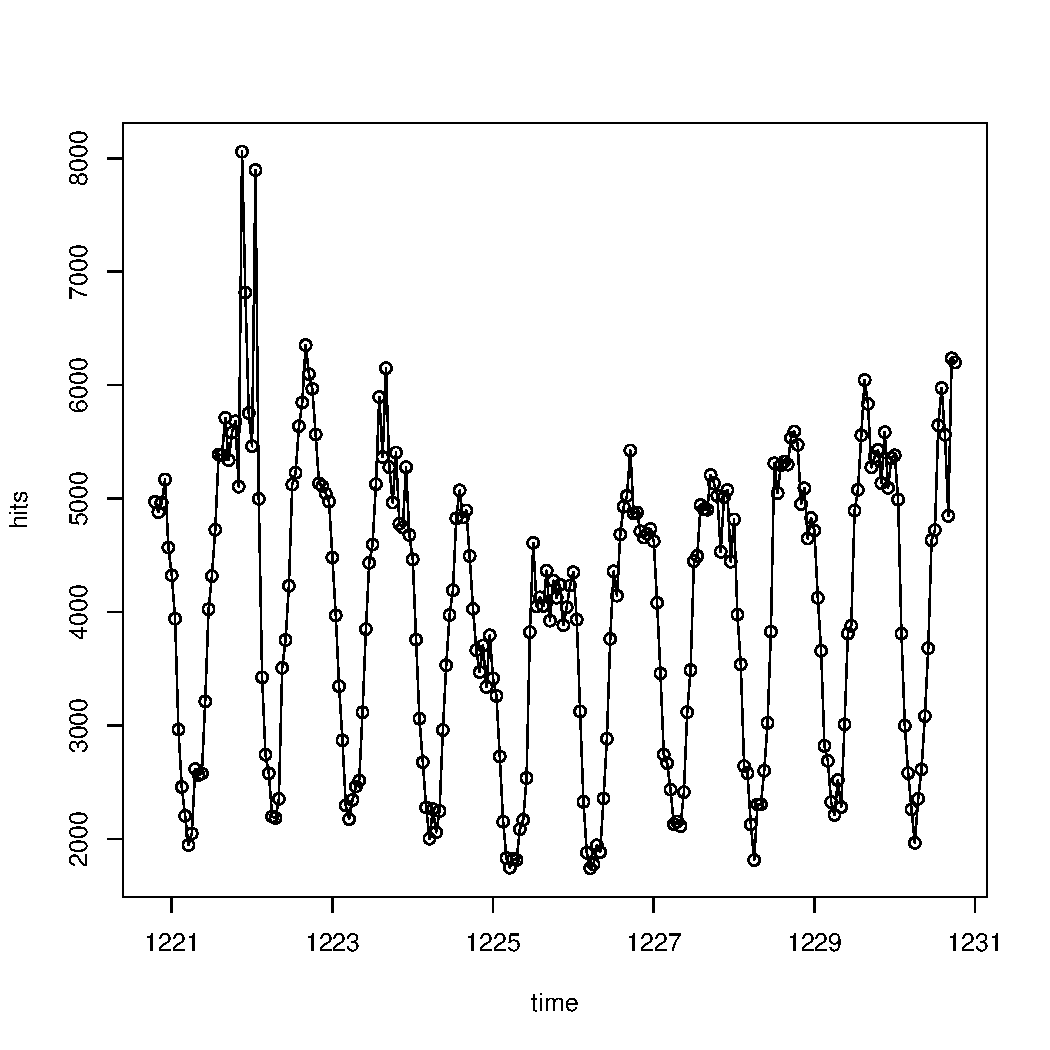
\includegraphics[width=\maxwidth]{figure/unnamed-chunk-5-1} 
\begin{kframe}\begin{alltt}
\hlcom{# dev.off()}
\end{alltt}
\end{kframe}
\end{knitrout}

\section{Q4}
\subsection{(a)}
\begin{knitrout}
\definecolor{shadecolor}{rgb}{0.969, 0.969, 0.969}\color{fgcolor}\begin{kframe}
\begin{alltt}
library(foreach)
require(parallel) 
require(doParallel)
nCores <- as.integer(Sys.getenv("SLURM_CPUS_ON_NODE"))
registerDoParallel(nCores)
library(stringr)
library(readr)

#Note: The single function and usuage of str_pad are refer from my classmate, Ming Qiu.
single <- function(filename)\{
  data <- readLines(filename)
  library(stringr)
  out <- data[str_detect(data,'Barack_Obama')]
  return(out) \}


n <- 960
#nsub <- 10
result <- foreach(
  i = 1:n,
  .packages = c("stringr"), 
  .combine = c,              
  .verbose = TRUE) %dopar% \{     
    filename <- paste("/global/scratch/paciorek/wikistats_full/dated_for_R/part-", str_pad(i-1, width=5, side="left", pad="0"),sep = "")
     #filename <- paste("C:/Users/Esther/Desktop/stat243-fall-2017-master/part-",str_pad(i-1, width=5, side="left", pad="0"),sep = "")
    outputs <- single(filename)
    #outputs
  \}

results <- data.frame (matrix(sapply(list(result),function(x) unlist(strsplit(x,split=" ") ) ), ncol=6, byrow = TRUE) )
#results <- data.frame ( t(sapply(result,function(x) unlist(strsplit(x,split=" ")) ) ))
colnames(results) <- c("date", "time", "language", "webpage", "number of hits", "page size")
head(results)
class(results)
print(dim(results))
proc.time()

\end{alltt}
\end{kframe}
\end{knitrout}
Part of output file is following:
\begin{knitrout}
\definecolor{shadecolor}{rgb}{0.969, 0.969, 0.969}\color{fgcolor}\begin{kframe}
\begin{alltt}
\hlstd{dic} \hlkwb{<-} \hlstr{"C:/Users/Esther/Desktop/stat243-fall-2017-master/section/s07/ps6q4no.out"}
\hlstd{output} \hlkwb{<-} \hlkwd{readLines}\hlstd{(dic)}
\hlkwd{tail}\hlstd{(output,} \hlnum{25}\hlstd{)}
\end{alltt}
\begin{verbatim}
##  [1] "      date   time  language                                            webpage"
##  [2] "1 20081231 100000 commons.m                    File:Barack_Obama_signature.svg"
##  [3] "2 20081202 150000        en Image:Michelle,_Oprah_Winfrey_and_Barack_Obama.jpg"
##  [4] "3 20081229 200001        en        Europe_and_Ireland_not_MYOB_or_Barack_Obama"
##  [5] "4 20081123 100000        it                           Discussione:Barack_Obama"
##  [6] "5 20081101 010000        pt                            Imagem:Barack_Obama.jpg"
##  [7] "6 20081231 120000        en                         Washington_Or_Barack_Obama"
##  [8] "  number of hits page size"                                                    
##  [9] "1              4     26796"                                                    
## [10] "2              2     19158"                                                    
## [11] "3              1      6047"                                                    
## [12] "4              1     40260"                                                    
## [13] "5              3     24840"                                                    
## [14] "6              1      6007"                                                    
## [15] "> class(results)"                                                              
## [16] "[1] \"data.frame\""                                                            
## [17] "> print(dim(results))"                                                         
## [18] "[1] 325263      6"                                                             
## [19] "> proc.time()"                                                                 
## [20] "     user    system   elapsed "                                                
## [21] "34664.559  2247.375  2715.079 "                                                
## [22] "> "                                                                            
## [23] "> proc.time()"                                                                 
## [24] "     user    system   elapsed "                                                
## [25] "34664.560  2247.375  2715.093 "
\end{verbatim}
\end{kframe}
\end{knitrout}
\subsection{(b)}
As the time is 2715 seconds(46 minutes) for one node, which vert close to 12 minutes if divide it my 4. Hence, using R for each has almost similar times or even faster.\\

\subsection{(c)}
\begin{knitrout}
\definecolor{shadecolor}{rgb}{0.969, 0.969, 0.969}\color{fgcolor}\begin{kframe}
\begin{alltt}
#statistic allicate
library(foreach)
require(parallel) 
require(doParallel)
nCores <- as.integer(Sys.getenv("SLURM_CPUS_ON_NODE"))
registerDoParallel(nCores)
library(stringr)

#Note: The single function and usuage of str_pad are refer from my classmate, Ming Qiu.
single <- function(filename)\{
  data <- readLines(filename)
  library(stringr)
  out <- data[str_detect(data,'Barack_Obama')]
  return(out) \}

n <- 960
#n <- 2
path <- "/global/scratch/paciorek/wikistats_full/dated_for_R/part-"
#path <- "C:/Users/Esther/Desktop/stat243-fall-2017-master/part-"
i=1:n
filename <- mclapply(n,  mc.preschedule=TRUE, function(x) paste(path,str_pad(i-1, width=5, side="left", pad="0"),sep = "")   )
output <- mclapply(filename[[1]], single,  mc.preschedule=TRUE)
results <- data.frame( matrix(sapply( unlist( output ), function(x) unlist(strsplit(x,split=" ") )), ncol=6, byrow = TRUE) )

colnames(results) <- c("date", "time", "language", "webpage", "number of hits", "page size")
head(results)
class(results)
print(dim(results))
proc.time()
write.table(results, file='/global/scratch/esther730/results_ob.csv',sep = ",",row.names = FALSE)
\end{alltt}
\end{kframe}
\end{knitrout}
The following output reveal the processing time of static allocate, which is 17198 that nearly 289 minutes, when running at 4 cores, it will cost nearly 71 minutes.
\begin{knitrout}
\definecolor{shadecolor}{rgb}{0.969, 0.969, 0.969}\color{fgcolor}\begin{kframe}
\begin{alltt}
\hlstd{dic} \hlkwb{<-} \hlstr{"C:/Users/Esther/Desktop/stat243-fall-2017-master/section/s07/ps6q4st.out"}
\hlstd{output} \hlkwb{<-} \hlkwd{readLines}\hlstd{(dic)}
\hlkwd{tail}\hlstd{(output,} \hlnum{25}\hlstd{)}
\end{alltt}
\begin{verbatim}
##  [1] "1                                                                                                                            Barack_Obama"
##  [2] "2 Special:AllPages/I_ran_Project_Vote_voter_registration_drive_in_Illinois,_ACORN_was_smack_dab_in_the_middle_of_it,%22_said_Barack_Obama"
##  [3] "3                                                                                                             Bilde:Barack_Obama_2004.jpg"
##  [4] "4                                                                                                   Early_life_and_career_of_Barack_Obama"
##  [5] "5                                                                                                                            Barack_Obama"
##  [6] "6                                                                                                                   Discuter:Barack_Obama"
##  [7] "  number of hits page size"                                                                                                               
##  [8] "1             86   2032215"                                                                                                               
##  [9] "2              2     25520"                                                                                                               
## [10] "3              1      7825"                                                                                                               
## [11] "4             16    760462"                                                                                                               
## [12] "5              4     55875"                                                                                                               
## [13] "6              1     20922"                                                                                                               
## [14] "> class(results)"                                                                                                                         
## [15] "[1] \"data.frame\""                                                                                                                       
## [16] "> print(dim(results))"                                                                                                                    
## [17] "[1] 433895      6"                                                                                                                        
## [18] "> proc.time()"                                                                                                                            
## [19] "    user   system  elapsed "                                                                                                              
## [20] "16643.04   343.28 17197.31 "                                                                                                              
## [21] "> write.table(results, file='/global/scratch/esther730/results_ob.csv',sep = \",\",row.names = FALSE)"                                    
## [22] "> "                                                                                                                                       
## [23] "> proc.time()"                                                                                                                            
## [24] "     user    system   elapsed "                                                                                                           
## [25] "16643.653   343.314 17197.955 "
\end{verbatim}
\end{kframe}
\end{knitrout}

\begin{knitrout}
\definecolor{shadecolor}{rgb}{0.969, 0.969, 0.969}\color{fgcolor}\begin{kframe}
\begin{alltt}
#dynamic allocate
library(foreach)
require(parallel) 
require(doParallel)
nCores <- as.integer(Sys.getenv("SLURM_CPUS_ON_NODE"))
registerDoParallel(nCores)
library(stringr)


single <- function(filename)\{
  data <- readLines(filename)
  library(stringr)
  out <- data[str_detect(data,'Barack_Obama')]
  return(out) \}


n <- 960
#nsub <- 10
result <- foreach(
  i = 1:n,
  .packages = c("stringr"), 
  .combine = c,              
  .verbose = TRUE) %dopar% \{     
    filename <- paste("/global/scratch/paciorek/wikistats_full/dated_for_R/part-", str_pad(i-1, width=5, side="left", pad="0"),sep = "")
    outputs <- mclapply(filename,single, mc.preschedule=FALSE)
    #outputs
  \}
results <- data.frame (matrix(sapply(list(result),function(x) unlist(strsplit(x,split=" ") ) ), ncol=6, byrow = TRUE) )
#results <- data.frame ( t(sapply(result,function(x) unlist(strsplit(x,split=" ")) ) ))
colnames(results) <- c("date", "time", "language", "webpage", "number of hits", "page size")
head(results)
class(results)
print(dim(results))
proc.time()
\end{alltt}
\end{kframe}
\end{knitrout}

The dynamic allocate used 22585 seconds(377minutes) to grep the strings among 960 files. When running on four nodes, it will cost about 94 minutes to obtain the results.
\begin{knitrout}
\definecolor{shadecolor}{rgb}{0.969, 0.969, 0.969}\color{fgcolor}\begin{kframe}
\begin{alltt}
\hlstd{dic} \hlkwb{<-} \hlstr{"C:/Users/Esther/Desktop/stat243-fall-2017-master/section/s07/ps6q4dy.out"}
\hlstd{output} \hlkwb{<-} \hlkwd{readLines}\hlstd{(dic)}
\hlkwd{tail}\hlstd{(output,} \hlnum{25}\hlstd{)}
\end{alltt}
\begin{verbatim}
##  [1] "1                                                                                                                            Barack_Obama"
##  [2] "2 Special:AllPages/I_ran_Project_Vote_voter_registration_drive_in_Illinois,_ACORN_was_smack_dab_in_the_middle_of_it,%22_said_Barack_Obama"
##  [3] "3                                                                                                             Bilde:Barack_Obama_2004.jpg"
##  [4] "4                                                                                                   Early_life_and_career_of_Barack_Obama"
##  [5] "5                                                                                                                            Barack_Obama"
##  [6] "6                                                                                                                   Discuter:Barack_Obama"
##  [7] "  number of hits page size"                                                                                                               
##  [8] "1             86   2032215"                                                                                                               
##  [9] "2              2     25520"                                                                                                               
## [10] "3              1      7825"                                                                                                               
## [11] "4             16    760462"                                                                                                               
## [12] "5              4     55875"                                                                                                               
## [13] "6              1     20922"                                                                                                               
## [14] "> class(results)"                                                                                                                         
## [15] "[1] \"data.frame\""                                                                                                                       
## [16] "> print(dim(results))"                                                                                                                    
## [17] "[1] 433895      6"                                                                                                                        
## [18] "> proc.time()"                                                                                                                            
## [19] "    user   system  elapsed "                                                                                                              
## [20] "43138.56  1849.43 22584.29 "                                                                                                              
## [21] "> #write.table(results, file='/global/scratch/esther730/results_ob.csv',sep = \",\",row.names = FALSE)"                                   
## [22] "> "                                                                                                                                       
## [23] "> proc.time()"                                                                                                                            
## [24] "    user   system  elapsed "                                                                                                              
## [25] "43138.56  1849.43 22584.30 "
\end{verbatim}
\end{kframe}
\end{knitrout}
Hence, generally, static allocation is better method than dynamic way in this case.

\section{Q5}


\end{document}
